
%%% Local Variables:
%%% mode: latex
%%% TeX-master: "main"
%%% End:

\chapter{The Propagation of Light}

\section{The Fresnel Equations}

\subsection{Electric Field Perpendicular to Plane of Incidence}

\begin{figure}[H]
  \centering
  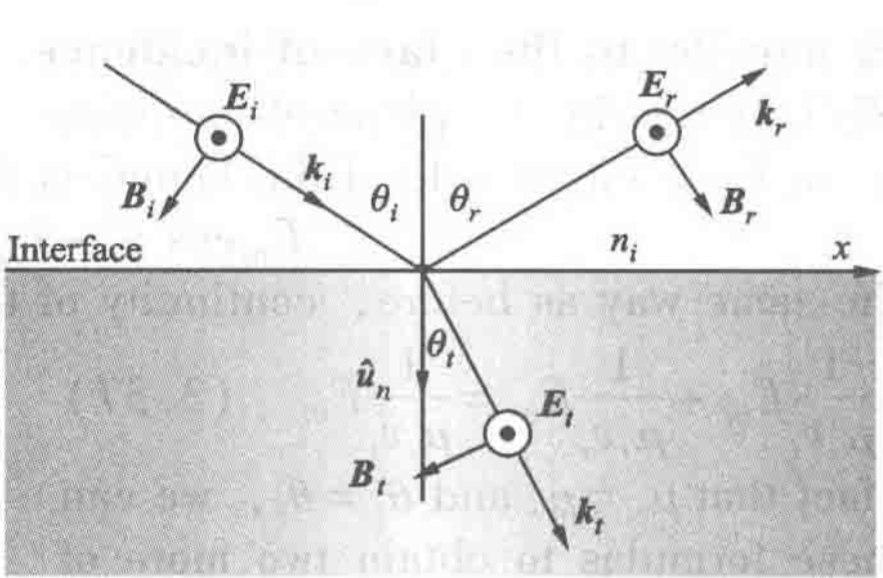
\includegraphics[width=0.5\linewidth]{figures/Fresnel-perpendicular}
  \label{fig:}
\end{figure}

\begin{equation*}
 \left\{
  \begin{aligned}
    & E_i + E_r = E_t \\
    & B_i \cos \theta_i = B_r \cos \theta_r + B_t \cos \theta_t
  \end{aligned}
  \right.
\end{equation*}

\begin{equation*}
  \left\{
  \begin{aligned}
    & E = v B \\
    & v = \dfrac{c}{n}
  \end{aligned}
  \right.
\end{equation*}

We define the amplitude reflection coefficient $r$, the amplitude transmission coefficient $t$

\begin{equation*}
  \begin{aligned}
    r = \dfrac{n_i \cos \theta_i - n_t \cos \theta_t}{n_i \cos \theta_i + n_t \cos \theta_t} \\
    t = \dfrac{2 n_i \cos \theta_i}{n_i \cos \theta_i + n_t \cos \theta_t} 
  \end{aligned}
\end{equation*}

Considered that $n_i \sin \theta_i = n_t \sin \theta_t$

\begin{equation*}
  \begin{aligned}
    r_{\perp} &= \dfrac{\sin \left( \theta_i - \theta_t \right)}{\sin \left( \theta_i + \theta_t \right)} \\
    t_{\perp} &= \dfrac{2 \sin \theta_t \cos \theta_i}{\sin \left( \theta_i + \theta_t \right)} 
  \end{aligned}
\end{equation*}

\subsection{Electric Field Parallel to Plane of Incidence}

\begin{figure}[H]
  \centering
  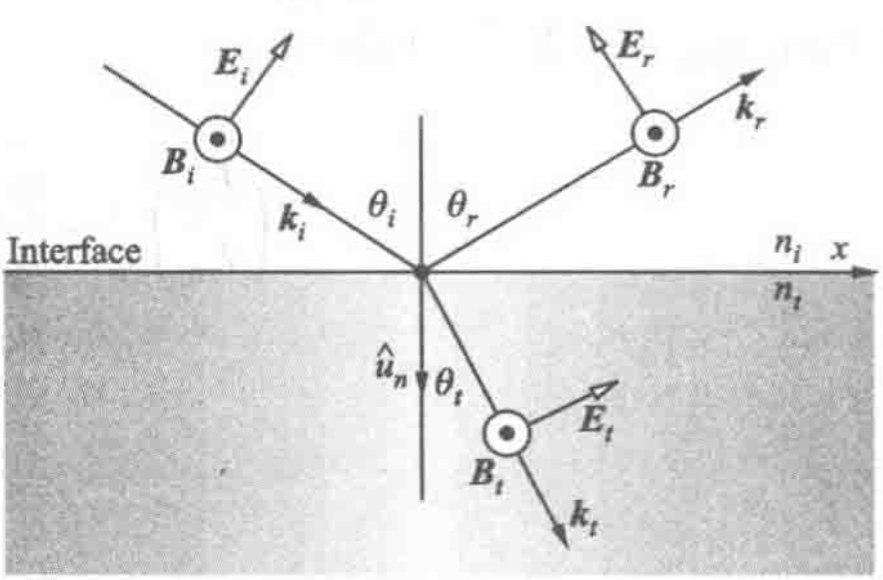
\includegraphics[width=0.5\linewidth]{figures/Fresnel-parallel}
  \label{fig:}
\end{figure}

\begin{equation*}
 \left\{
  \begin{aligned}
    & B_i + B_r = B_t \\
    & E_i \cos \theta_i = E_r \cos \theta_r + E_t \cos \theta_t
  \end{aligned}
  \right.
\end{equation*}

\begin{equation*}
  \left\{
  \begin{aligned}
    & E = v B \\
    & v = \dfrac{c}{n}
  \end{aligned}
  \right.
\end{equation*}

We define the amplitude reflection coefficient $r$, the amplitude transmission coefficient $t$

\begin{equation*}
  \begin{aligned}
    r = \dfrac{n_t \cos \theta_i - n_i \cos \theta_t}{n_t \cos \theta_i + n_i \cos \theta_t} \\
    t = \dfrac{2 n_i \cos \theta_i}{n_t \cos \theta_i + n_i \cos \theta_t} 
  \end{aligned}
\end{equation*}

Considered that $n_i \sin \theta_i = n_t \sin \theta_t$

\begin{equation*}
  \begin{aligned}
    r_{\parallel} &= \dfrac{\sin \left( 2 \theta_i \right) - \sin \left( 2 \theta_t \right)}{\sin \left( 2 \theta_i \right) + \sin \left( 2 \theta_t \right)} = \dfrac{\tan \left( \theta_i - \theta_t \right)}{\tan \left( \theta_i + \theta_t \right)} \\
    t_{\parallel} &= \dfrac{2 \sin \theta_t \theta_i}{\sin \left( \theta_i + \theta_t \right) \cos \left( \theta_i - \theta_t \right)} 
  \end{aligned}
\end{equation*}

\section{Polarization Angle}

\begin{equation*}
  \begin{aligned}
    \theta_p = \arctan \left( \dfrac{\theta_p}{\theta_i}  \right)
  \end{aligned}
\end{equation*}

\begin{figure}[H]
  \centering
  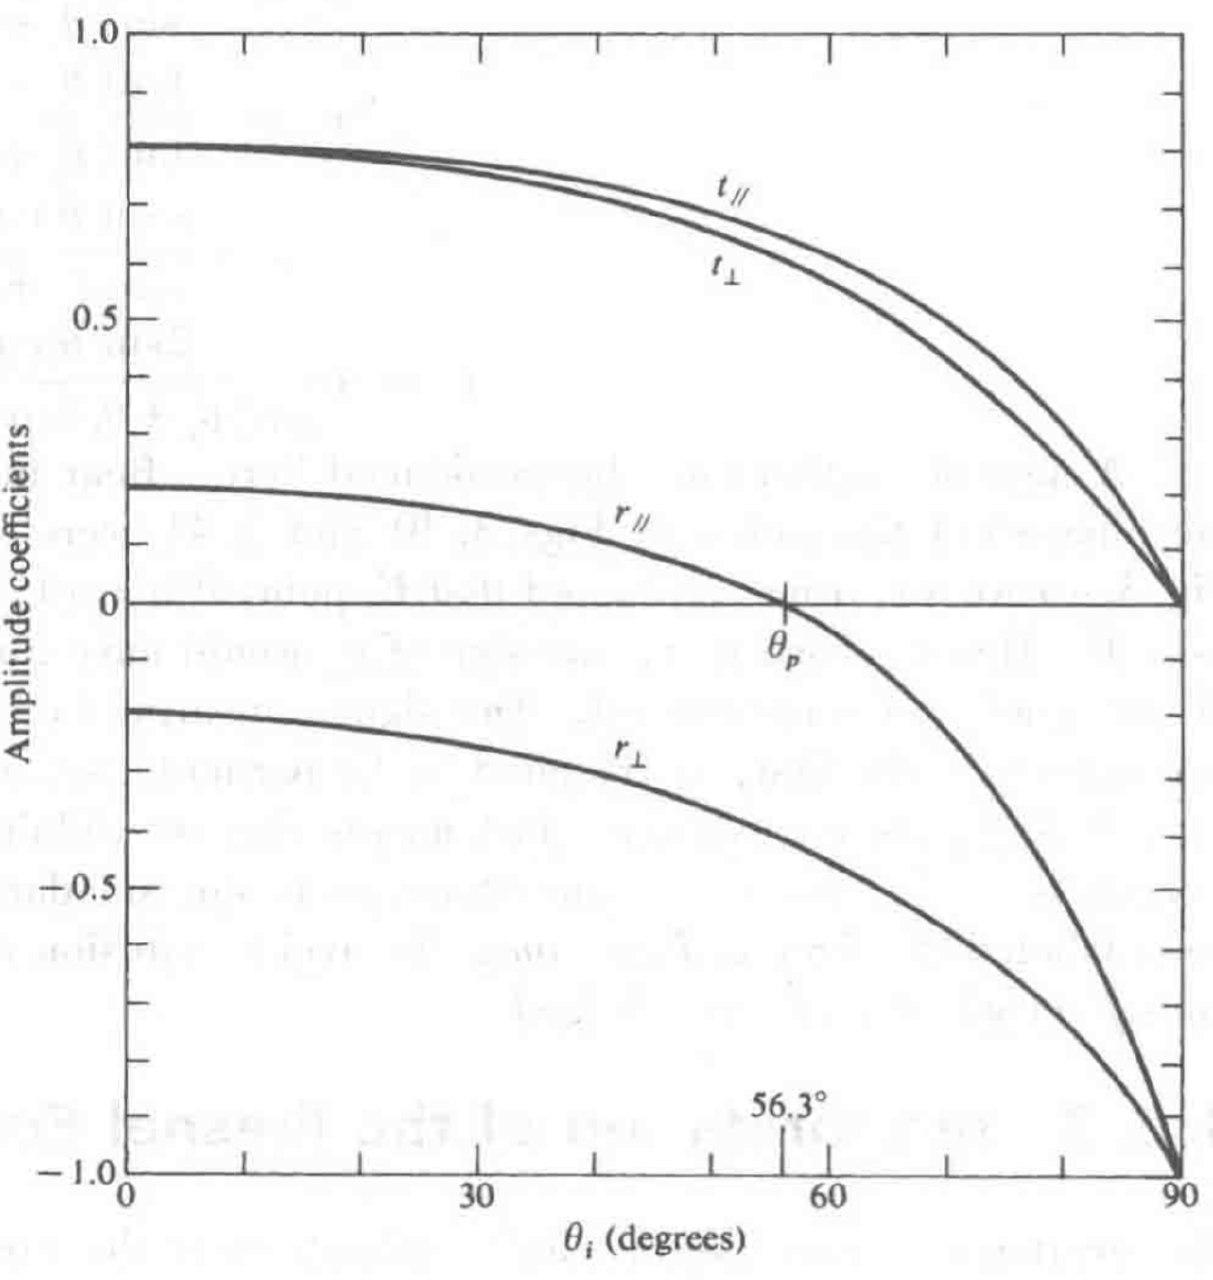
\includegraphics[width=0.3\linewidth]{figures/Polarization-angle}
  \label{fig:}
\end{figure}

\section{Critical Angle}

\begin{equation*}
  \begin{aligned}
    \theta_C = \arcsin \left( \dfrac{n_t}{n_i}  \right)
  \end{aligned}
\end{equation*}

